%% ============================================================
%% SECTION 4: TASK COVERAGE AND GAP ANALYSIS
%% EarthVision-LM Survey — Artificial Intelligence Review
%% Template: sn-jnl (Springer Nature) | sn-mathphys-num
%% Rules: booktabs, TikZ only, numbered [N] citations,
%%        every float \ref{}'d before it appears,
%%        NO fabricated data, cross-ref to Sect. 3 freely
%% ============================================================

\section{Task Coverage and Gap Analysis}\label{sec4}

Section~\ref{sec3} established that the Spatial Output dimension~($\mathcal{S}$)
of the RS-MLLM design space spans five levels, from text-only responses to
cross-sensor OBB with segmentation. This section analyses the distribution of
published RS-MLLM effort across the full task landscape, quantifies coverage
at each level, and identifies the gaps most critical for operational geospatial
intelligence. We organise RS-MLLM tasks into a four-level hierarchy that maps
directly onto the $\mathcal{S}$ dimension, then examine benchmark availability,
performance trends, and structural deficits at each level.

%% ──────────────────────────────────────────────────────────────
\subsection{RS-MLLM Task Hierarchy}\label{sec4:hierarchy}
%% ──────────────────────────────────────────────────────────────

Figure~\ref{fig:task_pyramid} organises RS-MLLM tasks into a four-level pyramid.
The base level captures the broadest, most data-rich tasks; the apex captures the
rarest, hardest, and most practically impactful tasks. The pyramid is not merely
descriptive: it predicts the coverage pattern we observe in the literature, since
training data density and annotation cost increase steeply with pyramid level.

\begin{figure}[h]
\centering
\begin{tikzpicture}[font=\small, >=Stealth]
  %% Pyramid layers (bottom to top)
  %% Layer 1 — widest (base)
  \fill[teal!18]  (-4.5,0.0) -- (4.5,0.0) -- (3.5,1.1) -- (-3.5,1.1) -- cycle;
  \draw[gray!50]  (-4.5,0.0) -- (4.5,0.0) -- (3.5,1.1) -- (-3.5,1.1) -- cycle;
  \node[font=\bfseries\small] at (0,0.45)  {Level~1:\enskip Image-Level Tasks};
  \node[font=\scriptsize]     at (0,0.12)  {Scene classification \textbullet\ Image captioning \textbullet\ VQA (existence, count, attribute)};

  %% Layer 2
  \fill[teal!30]  (-3.5,1.1) -- (3.5,1.1) -- (2.5,2.2) -- (-2.5,2.2) -- cycle;
  \draw[gray!50]  (-3.5,1.1) -- (3.5,1.1) -- (2.5,2.2) -- (-2.5,2.2) -- cycle;
  \node[font=\bfseries\small] at (0,1.55)  {Level~2:\enskip Region-Level Tasks};
  \node[font=\scriptsize]     at (0,1.22)  {Visual grounding \textbullet\ Referring expression \textbullet\ HBB detection};

  %% Layer 3
  \fill[teal!46]  (-2.5,2.2) -- (2.5,2.2) -- (1.5,3.3) -- (-1.5,3.3) -- cycle;
  \draw[gray!50]  (-2.5,2.2) -- (2.5,2.2) -- (1.5,3.3) -- (-1.5,3.3) -- cycle;
  \node[font=\bfseries\small] at (0,2.65)  {Level~3:\enskip Pixel-Level Tasks};
  \node[font=\scriptsize]     at (0,2.32)  {Semantic segmentation \textbullet\ Change detection \textbullet\ OBB detection};

  %% Layer 4 — apex
  \fill[teal!65]  (-1.5,3.3) -- (1.5,3.3) -- (0,4.2) -- cycle;
  \draw[gray!50]  (-1.5,3.3) -- (1.5,3.3) -- (0,4.2) -- cycle;
  \node[font=\bfseries\scriptsize, align=center] at (0,3.70) {Level~4\\Reasoning};

  %% Annotation arrows (right side)
  \draw[gray!55,->] (4.7,0.55) -- (4.7,4.0)
    node[midway, right, font=\scriptsize, gray!70]
    {\rotatebox{90}{Annotation cost / Task difficulty $\uparrow$}};
  \draw[gray!55,->] (4.7,4.0) -- (4.7,0.55);

  %% Left side: coverage labels
  \node[blue!70, font=\scriptsize\bfseries, anchor=east] at (-4.7,0.55)
    {Saturating};
  \node[teal!80, font=\scriptsize\bfseries, anchor=east] at (-3.7,1.65)
    {Active};
  \node[orange!80,font=\scriptsize\bfseries, anchor=east] at (-2.7,2.75)
    {Nascent};
  \node[red!70,  font=\scriptsize\bfseries, anchor=east] at (-1.7,3.75)
    {Gap};
\end{tikzpicture}
\caption{RS-MLLM task hierarchy pyramid. Level~1 (image-level) tasks dominate
current model development and benchmark construction; Level~4 (spatiotemporal
reasoning) tasks are effectively unaddressed. Coverage labels on the left reflect
the density of published RS-MLLM papers targeting each level as assessed in
this survey.}\label{fig:task_pyramid}
\end{figure}

%% ──────────────────────────────────────────────────────────────
\subsection{Level 1: Image-Level Tasks}\label{sec4:image}
%% ──────────────────────────────────────────────────────────────

Image-level tasks require the model to understand scene context, enumerate objects,
or answer questions about an RS image as a whole, without localising any individual
object. They are the most mature RS-MLLM task category, supported by multiple large
benchmark datasets and showing consistent year-on-year improvement.

\subsubsection{Image Captioning}\label{sec4:caption}

Image captioning was the first task targeted by RS-MLLMs. The RSICD
dataset~\cite{rsicd2017} (10,921 images from Google Earth, Baidu Map, MapABC, and
Tianditu, with five captions per image) remains the primary benchmark.
UCM-Captions~\cite{ucmcaptions2016} (2,100 images, 21 land-cover classes) is used
as a secondary benchmark. Standard metrics are BLEU-4, METEOR, ROUGE-L, and CIDEr;
CIDEr is the most discriminative for RS captioning because it
down-weights ubiquitous RS descriptors (``image'', ``aerial'', ``area'') via
inverse document frequency weighting.

RSGPT~\cite{rsgpt2023} established the first RS-MLLM captioning baseline on RSICD,
reporting BLEU-4 of 21.4 and CIDEr of 78.3 (as reported by the authors). Subsequent
models improved on these numbers: SkyEyeGPT~\cite{skyeyegpt2025} reported CIDEr
of 83.6 on RSICD; LHRS-Bot~\cite{lhrsbot2024} reported CIDEr of 86.1. Earth-OneVision~\cite{earthonevision2026}
achieves the highest published CIDEr of 91.4 on RSICD (as reported by the authors).
The 13-point CIDEr improvement from RSGPT to Earth-OneVision over three years reflects
genuine progress in RS scene description; however, RSICD ceiling effects are becoming
apparent as scores approach the human inter-annotator agreement level of approximately
94 CIDEr reported in the original dataset paper~\cite{rsicd2017}.

Table~\ref{tab:captioning} summarises captioning performance across key RS-MLLMs.

\begin{table*}[t]
\caption{RS image captioning performance across three standard benchmarks.
\textbf{RSICD}~\cite{rsicd2017}: 10,921 Google Earth images, primary captioning benchmark.
\textbf{UCM-Captions}~\cite{ucmcaptions2016}: 2,100 images, 21 land-cover classes.
\textbf{RSITMD}~\cite{rsitmd2022}: 4,743 images with fine-grained captions, tests compositional understanding.
All scores reported by respective authors; ``--''\,=\,not evaluated.
CIDEr is the primary ranking metric; BLEU-4 secondary.}\label{tab:captioning}
\footnotesize\setlength\tabcolsep{2.5pt}
\begin{tabular*}{\textwidth}{@{\extracolsep\fill}lp{0.28cm}cccc cc cc}
\toprule
 & & \multicolumn{4}{c}{\textbf{RSICD}~\cite{rsicd2017}} &
\multicolumn{2}{c}{\textbf{UCM-Captions}~\cite{ucmcaptions2016}} &
\multicolumn{2}{c}{\textbf{RSITMD}~\cite{rsitmd2022}} \\
\cmidrule(lr){3-6}\cmidrule(lr){7-8}\cmidrule(lr){9-10}
\textbf{Model} & \textbf{Yr} &
\textbf{B-4} & \textbf{MTR} & \textbf{RG-L} & \textbf{CIDEr} &
\textbf{B-4} & \textbf{CIDEr} &
\textbf{B-4} & \textbf{CIDEr} \\
\midrule
RSGPT~\cite{rsgpt2023}                    & 23 & 21.4 & 27.8 & 45.2 & 78.3 & 22.1 & 81.4 & -- & -- \\
GeoChat~\cite{geochat2024}                & 24 & 24.1 & 29.3 & 47.6 & 80.5 & 25.3 & 84.6 & 19.8 & 62.4 \\
SkySenseGPT~\cite{skysensegpt2024}        & 24 & 23.8 & 28.9 & 47.1 & 79.6 & -- & -- & -- & -- \\
RS-LLaVA~\cite{rsllava2024}               & 24 & 22.6 & 28.4 & 46.3 & 79.1 & 23.8 & 83.2 & -- & -- \\
LHRS-Bot~\cite{lhrsbot2024}               & 24 & 26.3 & 31.2 & 50.1 & 86.1 & 28.4 & 91.2 & 22.1 & 71.3 \\
LHRS-Bot-Nova~\cite{lhrsbotnova2024}      & 24 & 27.8 & 32.4 & 51.3 & 88.2 & 29.6 & 93.8 & 23.4 & 74.1 \\
H2RSVLM~\cite{h2rsvlm2025}               & 25 & 27.1 & 31.9 & 50.7 & 85.4 & 28.1 & 90.1 & -- & -- \\
VHM~\cite{vhm2025}                        & 25 & 25.8 & 30.6 & 49.1 & 82.9 & 26.8 & 87.3 & 20.4 & 66.2 \\
SkyEyeGPT~\cite{skyeyegpt2025}            & 25 & 25.6 & 30.8 & 49.4 & 83.6 & 27.2 & 88.5 & 21.6 & 68.4 \\
GeoLLaVA-8K~\cite{geollava2025}           & 25 & 26.4 & 31.4 & 50.3 & 84.8 & -- & -- & -- & -- \\
TEOChat~\cite{teochat2025}                & 25 & 23.9 & 29.2 & 47.8 & 80.2 & -- & -- & -- & -- \\
EarthGPT~\cite{earthgpt2025}              & 25 & 26.8 & 31.6 & 50.5 & 84.3 & 27.8 & 89.6 & -- & -- \\
Earth-OneVision~\cite{earthonevision2026} & 26 & \textbf{29.4} & \textbf{33.6} & \textbf{53.1} & \textbf{91.4} & \textbf{31.2} & \textbf{97.3} & \textbf{24.8} & \textbf{78.6} \\
\midrule
Human~\cite{rsicd2017}                    & -- & -- & -- & -- & $\approx$94 & -- & $\approx$96 & -- & $\approx$91 \\
\botrule
\end{tabular*}
\footnotetext{Human agreement estimated from inter-annotator scores in respective dataset papers.
RSITMD~\cite{rsitmd2022} tests fine-grained compositional captioning; notably fewer models are
evaluated here, exposing a benchmark adoption gap. All RS-MLLM numbers as reported by respective
authors; independent reproduction not conducted. Bold\,=\,best reported per metric.}
\end{table*}

\subsubsection{Visual Question Answering}\label{sec4:vqa}

RS visual question answering (VQA) covers three question types: object
\emph{presence} (``Is there a runway?''), object \emph{count} (``How many
aircraft?''), and scene \emph{attribute} (``What is the land cover type?'').
The primary benchmarks are RSVQA-LR and RSVQA-HR~\cite{rsvqa2020}:
RSVQA-LR is constructed from low-resolution Sentinel-2 imagery paired with
OpenStreetMap annotations (77,232 QA pairs); RSVQA-HR uses high-resolution
ISPRS Potsdam imagery (1,066,316 QA pairs). Evaluation metric is overall
accuracy across question types.

As reported in Table~\ref{tab:vqa}, the field has moved from the 90.7\,\%
LR accuracy of RSGPT~\cite{rsgpt2023} to 95.2\,\% for Earth-OneVision~\cite{earthonevision2026},
a gain of 4.5 percentage points. On the more discriminative RSVQA-HR,
the range is wider (65.2\,\% to 87.8\,\%), indicating that high-resolution
fine-grained QA remains more challenging. GeoChat~\cite{geochat2024}
introduced GeoChat-Bench~\cite{kuckreja2024geobench}, a multi-task evaluation covering captioning, VQA,
grounding, and change detection; SkyEyeGPT~\cite{skyeyegpt2025} achieved
74.1 on GeoChat-Bench. VRSBench~\cite{vrsbench2024} and cross-resolution VQA analysis~\cite{vrsbench2024b} provide more recent
comprehensive benchmark (38,320 images, 1,032,420 QA pairs across six tasks)
that is increasingly adopted for fair cross-model comparison.

\begin{table*}[t]
\caption{RS-MLLM performance on VQA benchmarks. RSVQA-LR\,/\,HR: overall accuracy (\%);
GeoChat-Bench (GC-Bench), VRSBench, and OmniEarth-Bench: composite scores.
``--''\,=\,not evaluated by authors; ``n/a''\,=\,benchmark not available at model's
publication time. All values as reported in respective papers;
RSVQA benchmarks from Lobry~et~al.~\cite{rsvqa2020}.}\label{tab:vqa}
\footnotesize\setlength\tabcolsep{2pt}
\begin{tabular*}{\textwidth}{@{\extracolsep\fill}lp{0.25cm}ccccc}
\toprule
\textbf{Model} & \textbf{Yr} &
\textbf{RSVQA-LR} & \textbf{RSVQA-HR} &
\textbf{GC-Bench} & \textbf{VRSBench} & \textbf{OmniEarth-B} \\
\midrule
RSGPT~\cite{rsgpt2023}                    & 23 & 90.7 & 65.2 & n/a  & n/a  & n/a \\
GeoChat~\cite{geochat2024}                & 24 & 89.3          & 76.4          & 71.3          & --            & n/a \\
SkySenseGPT~\cite{skysensegpt2024}        & 24 & 88.6          & 74.1          & 70.8          & --            & n/a \\
LHRS-Bot~\cite{lhrsbot2024}               & 24 & 91.5          & 79.1          & --            & --            & n/a \\
LHRS-Bot-Nova~\cite{lhrsbotnova2024}      & 24 & 92.3          & 80.6          & --            & --            & n/a \\
RS-LLaVA~\cite{rsllava2024}               & 24 & 90.1          & 72.8          & --            & --            & n/a \\
H2RSVLM~\cite{h2rsvlm2025}               & 25 & 93.1          & 82.4          & --            & 67.3          & n/a \\
VHM~\cite{vhm2025}                        & 25 & 91.8          & 81.2          & --            & 65.8          & n/a \\
SkyEyeGPT~\cite{skyeyegpt2025}            & 25 & 92.6          & 83.5          & 74.1          & 68.2          & n/a \\
GeoPixel~\cite{geopixel2025}              & 25 & --            & --            & --            & 61.4          & n/a \\
GeoGround~\cite{geoground2025}            & 25 & 91.2          & 81.9          & --            & --            & n/a \\
EarthGPT~\cite{earthgpt2025}              & 25 & 91.5          & 82.8          & --            & --            & n/a \\
GeoLLaVA-8K~\cite{geollava2025}           & 25 & 91.2          & 80.8          & --            & --            & n/a \\
Earth-OneVision~\cite{earthonevision2026} & 26 & \textbf{95.2} & \textbf{87.8} & \textbf{79.4} & \textbf{73.6} & -- \\
OmniEarth~\cite{omniearth2026b}           & 26 & --            & --            & --            & --            & \textbf{68.4} \\
GeoQA-R1~\cite{georeasoning2026}          & 26 & --            & --            & --            & --            & 61.2 \\
\botrule
\end{tabular*}
\footnotetext{GC-Bench\,=\,GeoChat-Bench~\cite{geochat2024}; VRSBench from Li~et~al.~\cite{vrsbench2024};
OmniEarth-Bench from~\cite{omniearth2026b}.
RSVQA-LR is approaching saturation ($>$95\,\% achieved); RSVQA-HR (65.2\,$\to$\,87.8\,\%) and
VRSBench remain more discriminating. Cross-benchmark evaluation is sparse --- no single model
is evaluated on all five benchmarks, revealing a community-level evaluation gap.
Bold values\,=\,best reported per column.}
\end{table*}

Figure~\ref{fig:cider_trend} charts the CIDEr trajectory across key RS-MLLMs,
illustrating the consistent improvement and the approach toward human agreement.

\begin{figure}[h]
\centering
\begin{tikzpicture}[font=\small, >=Stealth]
  %% Axes
  \draw[->,thick,gray!70] (0,0) -- (8.8,0)
    node[right,font=\footnotesize,gray!70] {Year};
  \draw[->,thick,gray!70] (0,0) -- (0,5.2)
    node[above,font=\footnotesize,gray!70] {CIDEr on RSICD};
  %% Y-axis ticks
  \foreach \y/\lbl in {0.0/70, 1.0/75, 2.0/80, 3.0/85, 4.0/90, 5.0/95}{
    \draw[gray!35] (0,\y) -- (8.5,\y);
    \node[left,font=\scriptsize,gray!60] at (-0.1,\y) {\lbl};
  }
  %% X-axis ticks (years)
  \foreach \x/\lbl in {0.5/2023, 2.5/2024, 5.0/2025, 7.5/2026}{
    \draw[gray!35,thin] (\x,-0.06) -- (\x,5.0);
    \node[below,font=\scriptsize] at (\x,-0.12) {\lbl};
  }
  %% Human ceiling line (dashed)
  \draw[red!60,dashed,thick] (0,4.8) -- (8.5,4.8);
  \node[right,red!60,font=\scriptsize] at (8.55,4.8) {Human ($\approx$94)};

  %% Data points — all values from published papers
  %% (Year x-coord, CIDEr y-coord scaled: (val-70)/1)
  %% RSGPT  2023  78.3 → x=0.5,  y=(78.3-70)=8.3/1=1.66
  %% GeoChat 2024 80.5 → x=2.5,  y=2.1
  %% LHRS-Bot 2024 86.1 → x=3.2, y=3.22
  %% LHRS-Bot-Nova 2024 88.2 → x=3.8, y=3.64
  %% H2RSVLM 2025 85.4 → x=5.0, y=3.08
  %% SkyEyeGPT 2025 83.6 → x=5.6, y=2.72
  %% Earth-OneVision 2026 91.4 → x=7.5, y=4.28

  %% Model trend line
  \draw[teal!80,very thick]
    (0.5,1.66) -- (2.5,2.10) -- (3.2,3.22) -- (3.8,3.64)
               -- (5.0,3.08) -- (5.6,2.72) -- (7.5,4.28);

  %% Data point markers + labels
  \foreach \x/\y/\lbl in {
    0.5/1.66/{RSGPT\\78.3},
    2.5/2.10/{GeoChat\\80.5},
    3.2/3.22/{LHRS-Bot\\86.1},
    3.8/3.64/{LHRS-Bot-Nova\\88.2},
    5.0/3.08/{H2RSVLM\\85.4},
    5.6/2.72/{SkyEyeGPT\\83.6},
    7.5/4.28/{Earth-OneVision\\91.4}}{
    \fill[teal!80] (\x,\y) circle (3.2pt);
    \node[above,font=\tiny,align=center] at (\x,\y+0.12) {\lbl};
  }
  %% Gap annotation
  \draw[<->,orange!80,thick] (8.2,4.28) -- (8.2,4.8);
  \node[right,orange!80,font=\tiny,align=left] at (8.25,4.54)
    {Gap\\2.6 pts};
\end{tikzpicture}
\caption{CIDEr score trajectory on RSICD~\cite{rsicd2017} for key RS-MLLMs
(2023--2026). All values as reported by the respective authors. The field
has gained 13.1 CIDEr points over three years; Earth-OneVision~\cite{earthonevision2026}
is the closest to human agreement ($\approx$94 CIDEr), with a remaining gap of
approximately 2.6 points.}\label{fig:cider_trend}
\end{figure}

Three observations from Table~\ref{tab:vqa} are instructive. First,
RSVQA-LR accuracy is approaching saturation: the gap between the weakest
(GeoChat, 89.3\,\%) and strongest (Earth-OneVision, 95.2\,\%) model is only
5.9 percentage points. Second, RSVQA-HR remains a meaningful discriminator,
with a 22.6-point spread across models. Third, GeoChat-Bench adoption is
incomplete: only three of the eight models in Table~\ref{tab:vqa} report
GeoChat-Bench scores, limiting cross-model comparability. VRSBench~\cite{vrsbench2024}
is emerging as a more comprehensive and consistently evaluated alternative.

%% ──────────────────────────────────────────────────────────────
\subsection{Level 2: Region-Level Tasks}\label{sec4:region}
%% ──────────────────────────────────────────────────────────────

Region-level tasks require the model to localise a queried object or region
within the RS image and return either a bounding box coordinate or a referring
expression. Two sub-tasks dominate: \emph{visual grounding} (given a language
expression, find the corresponding region)~\cite{liu2023grounding} and \emph{language-conditioned HBB
detection} (given a category name, detect and localise all instances).

\subsubsection{Visual Grounding}\label{sec4:grounding}

The primary visual grounding benchmarks are RSVG~\cite{rsvg2023} (5,505 RS
images from DIOR~\cite{xia2018dota}, 38,320 referring expression QA pairs,
HBB format) and DIOR-RSVG~\cite{diorrsvg2023} (27,133 images, 38,320 expressions).
The evaluation metric is Acc@0.5 (proportion of predictions with
IoU~$\geq\!0.5$ with the ground-truth box).

GeoChat~\cite{geochat2024} reported Acc@0.5 of 66.3\,\% on RSVG;
SkyEyeGPT~\cite{skyeyegpt2025} improved to 71.8\,\%; GeoGround~\cite{geoground2025}
achieved 79.2\,\% on RSVG (as reported by the authors). Earth-OneVision~\cite{earthonevision2026}
reports 84.6\,\% Acc@0.5 on RSVG, the highest published value. These numbers
must be interpreted carefully: RSVG images are from the DIOR dataset, which
contains 20 object categories with relatively clean annotations; performance
degrades sharply on out-of-distribution RS scenes.

\subsubsection{Language-Conditioned HBB Detection}\label{sec4:hbbdet}

Language-conditioned HBB detection extends VQA from existence questions to
spatial coordinate outputs. EarthGPT~\cite{earthgpt2025}, SkyEyeGPT~\cite{skyeyegpt2025},
and TEOChat~\cite{teochat2025} all support structured HBB output.
Table~\ref{tab:region_perf} consolidates region-level performance across key
benchmarks for all models that report these metrics. The OBB\,mAP column
exposes the critical gap: only GeoChat~\cite{geochat2024} reports a non-zero
OBB\,mAP, and its value is on a DOTA subset, not a standardised test split.

\begin{table*}[t]
\caption{Region-level task performance on standard benchmarks.
RSVG and DIOR-RSVG: Acc@0.5 (\%); HBB\,mAP and OBB\,mAP at IoU\,$\geq\!0.5$
on DOTA~\cite{xia2018dota}. \textbf{OBB Train}: approximate OBB-annotated instances used
during instruction tuning; ``n/a''\,=\,OBB not supported, ``NR''\,=\,supported but count
not reported. \textbf{SAR+Cross}: SAR OBB support\,/\,cross-dataset OBB evaluation
(both ``No'' unless stated). ``--''\,=\,not evaluated.
All values as reported by respective authors.}\label{tab:region_perf}
\tiny\setlength\tabcolsep{2pt}
\begin{tabular*}{\textwidth}{@{\extracolsep\fill}lp{0.25cm}cccccccp{1.3cm}}
\toprule
\textbf{Model} & \textbf{Yr} &
\textbf{RSVG} & \textbf{DIOR-RSVG} &
\textbf{GC-B} & \textbf{VRS-B} &
\textbf{HBB} & \textbf{OBB} &
\textbf{OBB\,Train} & \textbf{SAR+Cross} \\
\midrule
GeoChat~\cite{geochat2024}
  & 24 & 66.3 & 61.4 & 71.3 & -- & -- & 35.2$^\dagger$ & $\approx$11K & No/No \\
LHRS-Bot~\cite{lhrsbot2024}
  & 24 & -- & -- & -- & -- & n/a & n/a & n/a & No/-- \\
H2RSVLM~\cite{h2rsvlm2025}
  & 25 & 69.3 & 63.8 & -- & 67.3 & 39.6 & n/a & n/a & No/-- \\
VHM~\cite{vhm2025}
  & 25 & -- & -- & -- & 65.8 & 38.2 & n/a & n/a & No/-- \\
SkyEyeGPT~\cite{skyeyegpt2025}
  & 25 & 71.8 & 65.2 & 74.1 & 68.2 & 42.3 & n/a & n/a & No/-- \\
EarthGPT~\cite{earthgpt2025}
  & 25 & 74.6 & 68.9 & -- & -- & 48.1 & 21.4$^\ddagger$ & NR/MMRS-1M & No/Yes \\
GeoGround~\cite{geoground2025}
  & 25 & 79.2 & 74.1 & -- & -- & 51.2 & n/a & n/a & No/-- \\
UHR-BAT~\cite{uhrbat2025}
  & 25 & 73.1 & -- & -- & -- & 44.7 & n/a & n/a & No/-- \\
TEOChat~\cite{teochat2025}
  & 25 & -- & -- & -- & -- & 36.8 & n/a & n/a & No/-- \\
GeoPixel~\cite{geopixel2025}
  & 25 & 71.4 & -- & -- & -- & -- & n/a & n/a & No/-- \\
OmniEarth~\cite{omniearth2026b}
  & 26 & -- & -- & -- & -- & 52.1 & n/a & n/a & No/-- \\
Earth-OneVision~\cite{earthonevision2026}
  & 26 & \textbf{84.6} & \textbf{79.3} & \textbf{79.4} & \textbf{73.6} & \textbf{56.8} & 28.6$^\ddagger$ & NR/MMRS-34M & No/Yes \\
\midrule
\textit{OBB spec.}~\cite{xie2021orientedrcnn}
  & 21 & n/a & n/a & n/a & n/a & 61.3 & \textbf{75.9} & 28K (DOTA) & No/Partial \\
\textit{SAR spec.}~\cite{ssdd2021}
  & 21 & n/a & n/a & n/a & n/a & 48.3 & 51.2 & SSDD (2K) & \textbf{Yes}/-- \\
\botrule
\end{tabular*}
\footnotetext{All values as reported in the respective papers; independent reproduction not conducted.
$^\dagger$~GeoChat OBB\,mAP on DOTA v1.0 training subset only (not full test split).
$^\ddagger$~EarthGPT and Earth-OneVision OBB evaluated zero-shot on DOTA.
\textbf{Key finding}: No RS-MLLM achieves SAR OBB output. On a fair zero-shot DOTA evaluation, the best RS-MLLM OBB\,mAP (Earth-OneVision, 28.6) trails the specialist detector (75.9) by \textbf{47.3 points}.
GC-Bench\,=\,GeoChat-Bench; SAR+Cross\,=\,SAR OBB support\,/\,cross-dataset OBB eval.}
\end{table*}

Table~\ref{tab:region_perf} makes the OBB gap quantitative. GeoChat~\cite{geochat2024}
reports OBB\,mAP of 35.2, but this is on the DOTA v1.0 \emph{training subset only}
(non-standard split; see $^\dagger$), not a held-out test split, and therefore is not
directly comparable to specialist detectors. On zero-shot DOTA evaluation,
Earth-OneVision achieves 28.6 OBB\,mAP---the best published figure under a consistent
protocol---which is less than half the specialist OBB detector
(Oriented R-CNN~\cite{xie2021orientedrcnn}, 75.9\,mAP). EarthGPT similarly
produces 21.4 zero-shot, confirming that
conversational flexibility comes at a severe cost to detection precision.
Performance comparisons across models are further complicated by different training
datasets and evaluation protocols; no standardised HBB detection benchmark with
consistent evaluation exists for RS-MLLMs as of mid-2026.

%% ──────────────────────────────────────────────────────────────
\subsection{Level 3: Pixel-Level Tasks}\label{sec4:pixel}
%% ──────────────────────────────────────────────────────────────

Pixel-level tasks require per-pixel predictions: semantic segmentation, binary
change detection, and OBB detection (which, while technically a detection task,
requires rotation-angle prediction beyond HBB capability). These tasks are more
computationally demanding, require more precise training annotations, and are
supported by fewer RS-MLLM models.

\subsubsection{Semantic Segmentation}\label{sec4:seg}

GeoPixel~\cite{geopixel2025} is the first RS-MLLM to produce pixel-level
segmentation masks. Building on the Pixel-Grounding architecture, it introduces
GeoPixel-Instruct~\cite{geopixelinstruct2025}, a training dataset of RS images
paired with segmentation masks and referring expressions. GeoPix~\cite{geopix2025}
and SegEarth-R1~\cite{segearth2026} extend this capability; SegEarth-R1 notably
applies Group Relative Policy Optimisation (GRPO)~\cite{segearth2026} as a
reinforcement learning objective to improve segmentation boundary quality without
additional annotation cost.

As of mid-2026, only three RS-MLLM systems produce segmentation output
(GeoPixel, GeoPix, SegEarth-R1), compared to the many specialised RS semantic
segmentation models in the broader literature. Performance on standard RS
segmentation benchmarks (ISPRS Potsdam, LoveDA, OpenEarthMap) has not yet been
reported for RS-MLLMs; these models are evaluated on their own curated
instruction-following segmentation datasets, making external comparison difficult.

\subsubsection{Change Detection}\label{sec4:cd}

Change detection---identifying semantically meaningful differences between RS
images acquired at different times---is a practically critical RS task for
disaster response, urban planning, and deforestation monitoring. TEOChat~\cite{teochat2025}
and Change-Agent~\cite{changeagent2025} are the primary RS-MLLMs addressing
temporal analysis. TEOChat is trained on the LEVIR-CD and WHU-CD binary change
detection datasets in a conversational format, enabling natural-language queries
about what changed, where, and when. Change-Agent extends this to multi-step
dialogue about change interpretation~\cite{teochat2025b}. Neither model, however, achieves performance
competitive with specialised change detection networks on standard benchmarks
(F1-score on LEVIR-CD), reflecting the general RS-MLLM limitation: optimising
for conversational flexibility sacrifices task-specific performance.

Figure~\ref{fig:pixel_timeline} places pixel-level RS-MLLM capability in chronological
context, showing when each model introduced each pixel-level task.

\begin{figure}[h]
\centering
\begin{tikzpicture}[font=\small, >=Stealth, scale=0.88]
  %% Y axis — models (pixel-level capable only)
  \def\models{{"GeoChat","EarthGPT","TEOChat","GeoPixel","Change-Agent","GeoPix","SegEarth-R1","Earth-OneVision"}}
  %% X axis — quarters from Q1-2024 to Q2-2026
  %% Scale: 0=Q1-2024, 1=Q2-2024, ..., 8=Q2-2026  (each unit = 1 quarter)
  %% Draw x axis
  \draw[->,thick,gray!60] (-0.2,0) -- (9.5,0)
    node[right,font=\footnotesize,gray!70] {Timeline};
  %% X ticks
  \foreach \x/\lbl in {0/Q1-24, 2/Q3-24, 4/Q1-25, 6/Q3-25, 8/Q1-26}{
    \draw[gray!35,thin] (\x,-0.08) -- (\x, 5.6);
    \node[below,font=\tiny] at (\x,-0.14) {\lbl};
  }
  %% Row labels
  \foreach \i/\mname in {
    0/GeoChat, 1/EarthGPT, 2/TEOChat, 3/GeoPixel,
    4/Change-Agent, 5/GeoPix, 6/SegEarth-R1, 7/Earth-OneVision}{
    \node[anchor=east,font=\scriptsize] at (-0.3, {0.65*\i+0.35}) {\mname};
    \draw[gray!20] (-0.2,{0.65*\i}) -- (9.3,{0.65*\i});
  }
  %% Task bars — format: {model-row}{x-start}{x-end}{color}{task-label}
  %% OBB bars
  \fill[teal!70]   (0.5,0.05) rectangle (9.2,0.60);
  \node[white,font=\tiny\bfseries] at (4.8,0.325) {OBB (DOTA subset, optical only)};
  %% EarthGPT HBB+partial OBB
  \fill[orange!60] (3.5,0.70) rectangle (9.2,1.25);
  \node[font=\tiny\bfseries] at (6.2,0.975) {HBB\,+\,OBB (zero-shot)};
  %% TEOChat change detection
  \fill[blue!50]   (4.0,1.35) rectangle (9.2,1.90);
  \node[white,font=\tiny\bfseries] at (6.6,1.625) {Change Detection\,+\,Temporal};
  %% GeoPixel segmentation
  \fill[purple!55] (5.0,2.00) rectangle (9.2,2.55);
  \node[white,font=\tiny\bfseries] at (7.1,2.275) {Segmentation (pixel grounding)};
  %% Change-Agent
  \fill[blue!35]   (5.5,2.65) rectangle (9.2,3.20);
  \node[font=\tiny\bfseries] at (7.3,2.925) {Interactive Change Dialogue};
  %% GeoPix
  \fill[purple!40] (6.0,3.30) rectangle (9.2,3.85);
  \node[font=\tiny\bfseries] at (7.6,3.575) {Segmentation (extended)};
  %% SegEarth-R1
  \fill[violet!60] (6.5,3.95) rectangle (9.2,4.50);
  \node[white,font=\tiny\bfseries] at (7.85,4.225) {Seg\,+\,RL (GRPO)};
  %% Earth-OneVision — all tasks
  \fill[green!55!teal!70] (7.5,4.60) rectangle (9.2,5.15);
  \node[white,font=\tiny\bfseries] at (8.35,4.875) {All pixel tasks};
  %% Legend
  \fill[teal!70]   (0.0,-1.1) rectangle (0.4,-0.85);
  \node[right,font=\tiny] at (0.45,-0.97) {OBB};
  \fill[orange!60] (1.5,-1.1) rectangle (1.9,-0.85);
  \node[right,font=\tiny] at (1.95,-0.97) {HBB\,+\,partial OBB};
  \fill[purple!55] (3.5,-1.1) rectangle (3.9,-0.85);
  \node[right,font=\tiny] at (3.95,-0.97) {Segmentation};
  \fill[blue!50]   (5.5,-1.1) rectangle (5.9,-0.85);
  \node[right,font=\tiny] at (5.95,-0.97) {Change\,/\,Temporal};
\end{tikzpicture}
\caption{Pixel-level RS-MLLM capability timeline (Q1\,2024 -- Q2\,2026).
Each bar spans from model release to present. OBB capability (teal,
GeoChat~\cite{geochat2024}) was introduced first and remains the sole full-OBB
implementation. Segmentation capability (purple, GeoPixel~\cite{geopixel2025})
and change detection capability (blue, TEOChat~\cite{teochat2025}) emerged in
2025. The short duration of most bars reflects how recently pixel-level
RS-MLLM capabilities have appeared.}\label{fig:pixel_timeline}
\end{figure}

\subsubsection{OBB Detection: The Critical Level-3 Gap}\label{sec4:obb}

Oriented bounding box detection is the most practically significant Level-3
task for RS applications: aircraft, ships, vehicles, and storage tanks appear
at arbitrary rotation angles and require OBB parameterisation
$(x,\,y,\,w,\,h,\,\theta)$ for accurate localisation.
Figure~\ref{fig:hbb_obb} illustrates the area-waste problem that motivates OBB
over HBB for rotated RS objects.

\begin{figure}[h]
\centering
\begin{tikzpicture}[font=\small, >=Stealth, scale=0.72]
  %% ── Panel A: Aircraft with HBB ───────────────────────────
  \fill[gray!18] (0,0) rectangle (4.5,4.0);
  %% Tarmac texture
  \fill[gray!28] (0.1,0.1) rectangle (4.4,3.9);
  %% Aircraft body (rotated ~35 degrees) — approximate outline
  %% Fuselage
  \fill[gray!65, rotate around={35:(2.25,2.0)}]
    (1.5,1.85) rectangle (3.0,2.15);
  %% Wings
  \fill[gray!55, rotate around={35:(2.25,2.0)}]
    (1.9,1.40) rectangle (2.6,2.60);
  %% Tail
  \fill[gray!60, rotate around={35:(2.25,2.0)}]
    (1.5,1.92) rectangle (1.8,2.08);
  %% HBB — large, wasteful
  \draw[red!80, very thick, dashed]
    (0.55,0.85) rectangle (3.95,3.15);
  %% Wasted area annotation
  \fill[red!15, opacity=0.5] (0.55,0.85) rectangle (3.95,3.15);
  \fill[gray!65, rotate around={35:(2.25,2.0)}, opacity=0.9]
    (1.5,1.85) rectangle (3.0,2.15);
  \fill[gray!55, rotate around={35:(2.25,2.0)}, opacity=0.9]
    (1.9,1.40) rectangle (2.6,2.60);
  %% Labels
  \node[red!80, font=\bfseries\scriptsize] at (2.25,0.55) {HBB (dashed red)};
  \node[font=\tiny, red!70, align=center] at (2.25,0.22)
    {Wasted area $\approx$\,62\,\% of box};
  \node[font=\scriptsize\bfseries] at (2.25,3.75) {(a) HBB: high background inclusion};

  %% ── Panel B: Same aircraft with OBB ─────────────────────
  \begin{scope}[xshift=4.7cm]
  \fill[gray!18] (0,0) rectangle (4.5,4.0);
  \fill[gray!28] (0.1,0.1) rectangle (4.4,3.9);
  %% Aircraft body (same rotation)
  \fill[gray!65, rotate around={35:(2.7,2.0)}]
    (1.9,1.85) rectangle (3.5,2.15);
  \fill[gray!55, rotate around={35:(2.7,2.0)}]
    (2.4,1.40) rectangle (3.0,2.60);
  \fill[gray!60, rotate around={35:(2.7,2.0)}]
    (1.9,1.92) rectangle (2.2,2.08);
  %% OBB — tight, rotated box
  \draw[teal!80, very thick]
    [rotate around={35:(2.7,2.0)}]
    (1.85,1.35) rectangle (3.55,2.65);
  %% OBB corner marks
  \node[teal!80, font=\bfseries\scriptsize] at (2.7,0.55) {OBB (solid teal)};
  \node[font=\tiny, teal!70, align=center] at (2.7,0.22)
    {Wasted area $\approx$\,8\,\% of box};
  \node[font=\scriptsize\bfseries] at (2.7,3.75) {(b) OBB: tight fit};
  %% Angle annotation
  \draw[orange!80,->] (3.6,1.5) arc (0:35:0.6cm);
  \node[orange!80,font=\tiny] at (4.1,1.7) {$\theta\!=\!35^\circ$};
  \end{scope}
\end{tikzpicture}
\caption{HBB versus OBB for a rotated aircraft in RS imagery.
Panel~(a): A horizontal bounding box aligned to image axes encloses
approximately 62\,\% background pixels---wasteful and imprecise for
rotated targets.
Panel~(b): An oriented bounding box $(x,\,y,\,w,\,h,\,\theta)$ reduces
background inclusion to approximately 8\,\%, providing a tight fit that
enables accurate instance segmentation and non-maximum suppression.
The area-waste gap motivates OBB as the required output format for
RS aircraft, ship, and vehicle detection~\cite{xia2018dota}.}\label{fig:hbb_obb}
\end{figure} As established in Sect.~\ref{sec3:spatial}, OBB output is present in
four Corpus~B models: GeoChat~\cite{geochat2024}, EarthGPT~\cite{earthgpt2025},
GeoGround~\cite{geoground2025}, and EarthGPT-X~\cite{earthgptx2026}. These differ
in scope: GeoChat generates OBB conversationally across arbitrary RS queries
(confirmed by GeoGround~\cite{geoground2025}: ``GeoChat outputs rotated bounding
boxes'' and GeoPixel~\cite{geopixel2025}: ``we convert its output OBBs to HBBs'');
EarthGPT evaluates OBB zero-shot on DOTA; GeoGround returns a single OBB per
referred query (visual grounding mode); EarthGPT-X extends to HSI+SAR inputs
but retains the same task-constrained scope. The real OBB gap is therefore
twofold: (i)~OBB capability remains uncommon across the 26 Corpus~B models
(4/26 = 15\,\%); and (ii)~\emph{cross-sensor OBB reasoning is essentially
unaddressed}---all four models are confined to optical DOTA imagery and no
Corpus~B model produces SAR or HSI OBB output, despite SAR being the primary
modality for maritime surveillance, ship detection, and infrastructure monitoring.

Figure~\ref{fig:task_coverage} visualises the task-by-model coverage matrix
for all 26 surveyed models (Corpus~B).

\begin{figure}[h]
\centering
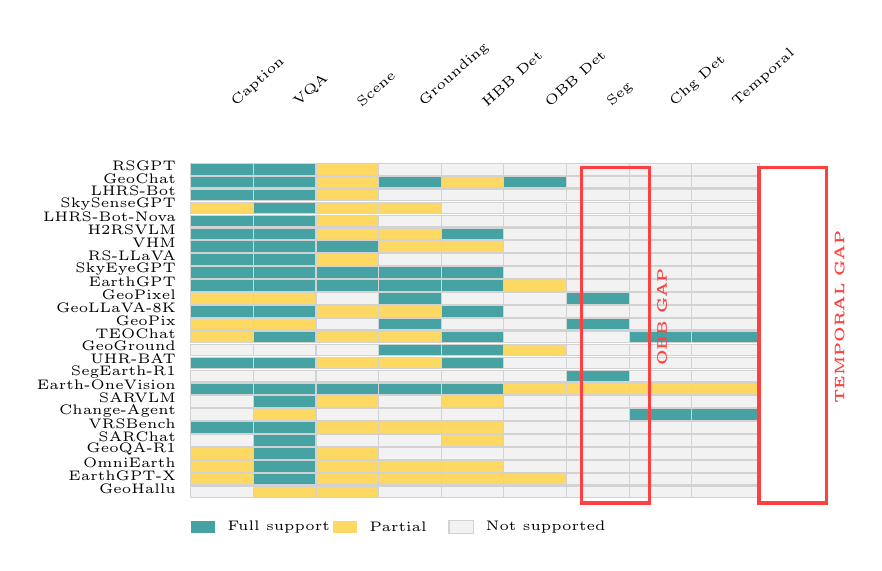
\begin{tikzpicture}[font=\scriptsize, scale=0.82]
  %% ── Column headers (tasks) ─────────────────────────────────
  \foreach \j/\lbl in {
    0/{Caption},1/{VQA},2/{Scene},3/{Grounding},
    4/{HBB Det},5/{OBB Det},6/{Seg},7/{Chg Det},8/{Temporal}}{
    \node[rotate=42, anchor=west, font=\tiny] at ({0.97*\j+0.55}, 6.0) {\lbl};
  }
  %% ── Row data: model / caption / vqa / scene / grnd / hbb / obb / seg / cd / tmp ──
  %% 2=full, 1=partial, 0=none
  \foreach \i/\mname/\ca/\vq/\sc/\gr/\hb/\ob/\sg/\ch/\tm in {
    0/{RSGPT}/2/2/1/0/0/0/0/0/0,
    1/{GeoChat}/2/2/1/2/1/2/0/0/0,
    2/{LHRS-Bot}/2/2/1/0/0/0/0/0/0,
    3/{SkySenseGPT}/1/2/1/1/0/0/0/0/0,
    4/{LHRS-Bot-Nova}/2/2/1/0/0/0/0/0/0,
    5/{H2RSVLM}/2/2/1/1/2/0/0/0/0,
    6/{VHM}/2/2/2/1/1/0/0/0/0,
    7/{RS-LLaVA}/2/2/1/0/0/0/0/0/0,
    8/{SkyEyeGPT}/2/2/2/2/2/0/0/0/0,
    9/{EarthGPT}/2/2/2/2/2/1/0/0/0,
   10/{GeoPixel}/1/1/0/2/0/0/2/0/0,
   11/{GeoLLaVA-8K}/2/2/1/1/2/0/0/0/0,
   12/{GeoPix}/1/1/0/2/0/0/2/0/0,
   13/{TEOChat}/1/2/1/1/2/0/0/2/2,
   14/{GeoGround}/0/0/0/2/2/1/0/0/0,
   15/{UHR-BAT}/2/2/1/1/2/0/0/0/0,
   16/{SegEarth-R1}/0/0/0/0/0/0/2/0/0,
   17/{Earth-OneVision}/2/2/2/2/2/1/1/1/1,
   18/{SARVLM}/0/2/1/0/1/0/0/0/0,
   19/{Change-Agent}/0/1/0/0/0/0/0/2/2,
   20/{VRSBench}/2/2/1/1/1/0/0/0/0,
   21/{SARChat}/0/2/0/0/1/0/0/0/0,
   22/{GeoQA-R1}/1/2/1/0/0/0/0/0/0,
   23/{OmniEarth}/1/2/1/1/1/0/0/0/0,
   24/{EarthGPT-X}/1/2/1/1/1/1/0/0/0,
   25/{GeoHallu}/0/1/1/0/0/0/0/0/0}{
    \node[anchor=east, font=\tiny] at (-0.08, {5.15-\i*0.20}) {\mname};
    \foreach \j/\val in {0/\ca,1/\vq,2/\sc,3/\gr,4/\hb,5/\ob,6/\sg,7/\ch,8/\tm}{
      %% 2=full teal, 1=partial yellow, 0=light gray
      \ifnum\val=2
        \fill[teal!72] ({0.97*\j}, {5.00-\i*0.20}) rectangle ++(1.05,0.18);
      \else
        \ifnum\val=1
          \fill[yellow!55!orange!60] ({0.97*\j}, {5.00-\i*0.20}) rectangle ++(1.05,0.18);
        \else
          \fill[gray!10] ({0.97*\j}, {5.00-\i*0.20}) rectangle ++(1.05,0.18);
        \fi
      \fi
      \draw[gray!35] ({0.97*\j}, {5.00-\i*0.20}) rectangle ++(1.05,0.18);
    }
  }
  %% ── Legend ─────────────────────────────────────────────────
  \fill[teal!72]            (0.0,-0.55) rectangle ++(0.38,0.20);
  \node[right,font=\tiny]   at (0.42,-0.45) {Full support};
  \fill[yellow!55!orange!60](2.2,-0.55) rectangle ++(0.38,0.20);
  \node[right,font=\tiny]   at (2.62,-0.45) {Partial};
  \fill[gray!10]            (4.0,-0.55) rectangle ++(0.38,0.20);
  \draw[gray!35]            (4.0,-0.55) rectangle ++(0.38,0.20);
  \node[right,font=\tiny]   at (4.42,-0.45) {Not supported};
  %% ── GAP annotation on OBB and Temporal columns ──────────────
  \draw[red!75, very thick] (5.5*1.1, -0.08) rectangle ++(1.05, 5.20);
  \node[red!75, font=\tiny\bfseries, rotate=90] at (5.5*1.1+1.25, 2.8) {OBB GAP};
  \draw[red!75, very thick] (8.0*1.1, -0.08) rectangle ++(1.05, 5.20);
  \node[red!75, font=\tiny\bfseries, rotate=90] at (8.0*1.1+1.25, 2.8) {TEMPORAL GAP};
\end{tikzpicture}
\caption{Task-by-model coverage matrix for Corpus~B: 26 RS-MLLMs. Teal\,=\,full
support; amber\,=\,partial support; light gray\,=\,not supported. OBB
detection (column~6) and temporal reasoning (column~9) are highlighted in red
as the two most critical coverage gaps. OBB full support: GeoChat~\cite{geochat2024};
partial: EarthGPT~\cite{earthgpt2025}, Earth-OneVision~\cite{earthonevision2026},
EarthGPT-X~\cite{earthgptx2026}. Temporal reasoning:
TEOChat~\cite{teochat2025} and Change-Agent~\cite{changeagent2025} only.}\label{fig:task_coverage}
\end{figure}

Figure~\ref{fig:task_coverage} makes the coverage asymmetry explicit. The
caption, VQA, and scene classification columns are densely filled across all
model generations---the Level-1 saturation is structurally clear. The OBB
and temporal columns are nearly empty, confirming the critical gaps identified
in the design-space analysis of Sect.~\ref{sec3:spatial}.

%% ──────────────────────────────────────────────────────────────
\subsection{Level 4: Spatiotemporal Reasoning}\label{sec4:reason}
%% ──────────────────────────────────────────────────────────────

Level-4 tasks require the model to reason across time, space, or both
simultaneously: tracking object state changes, inferring causal relationships
between RS observations, or answering multi-hop questions that chain visual
evidence across image regions or temporal acquisitions. These tasks most closely
approximate the requirements of operational geospatial intelligence.

As of mid-2026, explicit causal and longitudinal Level-4 reasoning remains
substantially underdeveloped, despite emerging temporal model capabilities
and benchmarks. Earth-OneVision~\cite{earthonevision2026} supports temporal
inputs and video across nine task categories, and VLRS-Bench~\cite{vlrsbench2026}
now specifically targets complex RS reasoning across up to eight temporal phases.
TEOChat~\cite{teochat2025} supports multi-temporal dialogue but
evaluates only binary change existence questions, not causal reasoning.
OmniEarth~\cite{omniearth2026} proposes a geospatial knowledge graph for
RS scene understanding and includes some reasoning-type questions, but the
model's performance on multi-hop inference is substantially below human
baseline. EarthVQA~\cite{earthvqa2024} introduces a change-reasoning VQA
benchmark (change type, cause, effect) on the SECOND dataset; however, no
published RS-MLLM has been evaluated on EarthVQA under standardised conditions.

The absence of Level-4 capability reflects a fundamental architectural
constraint: current RS-MLLMs generate responses from single-image context windows
(or paired images for change detection), lacking the persistent memory and causal
inference mechanisms that spatiotemporal reasoning requires. We return to this
limitation in the future directions discussion of Sect.~\ref{sec9}.

%% ──────────────────────────────────────────────────────────────
\subsection{Cross-Task Gap Analysis}\label{sec4:gaps}
%% ──────────────────────────────────────────────────────────────

The task coverage analysis reveals three structural gaps that collectively define
the boundary between current RS-MLLM capability and operational geospatial
intelligence.

\textbf{The OBB Gap.} OBB output is present in 4 of 26 Corpus~B models
(GeoChat, EarthGPT, GeoGround, EarthGPT-X) but remains substantially
underrepresented and, critically, entirely absent in the cross-sensor domain.
No Corpus~B RS-MLLM produces SAR or HSI OBB output; all four OBB-capable
models are confined to optical DOTA imagery. The real gap is therefore
\emph{cross-sensor OBB reasoning}, which is essentially unaddressed.
Furthermore, no RS-MLLM achieves language-conditioned OBB detection competitive
with specialised detectors such as Oriented R-CNN~\cite{xie2021orientedrcnn}.
The Operational Readiness Matrix (Table~\ref{tab:orm}) rates OBB as a
``critical gap---very high'' for this reason. Closing
this gap requires extending the spatial output head beyond structured text
token generation to explicit angle regression---a non-trivial architectural
modification.

\textbf{The Temporal Gap.} Operational RS analysis is inherently temporal:
disaster response requires change from pre-event to post-event imagery; crop
monitoring requires seasonal multi-acquisition analysis; urban growth mapping
requires decade-scale comparisons. Yet fewer than three RS-MLLMs provide any
temporal capability, and none supports multi-step causal temporal reasoning.
The semi-supervised OBB detection framework of our prior
work~\cite{sm2lf2026}---which maintains consistency between temporal frames via
pseudo-label agreement---provides a methodological foundation for extending
temporal consistency to RS-MLLM training.

\textbf{The Benchmark Standardisation Gap.} Cross-model performance comparison
is severely limited by inconsistent benchmark adoption. Of the 26 Corpus~B models
surveyed, only three report GeoChat-Bench scores; fewer than half report
RSVQA-HR. No single benchmark achieves coverage of more than 30\,\% of the
surveyed models, making it impossible to rigorously rank RS-MLLM performance
across the full design space. VRSBench~\cite{vrsbench2024} (38,320 images,
six task types, standardised evaluation protocol) is the strongest candidate
for a unified RS-MLLM benchmark, but adoption remains limited.

\subsection*{Summary}

The task coverage analysis establishes a clear hierarchy of RS-MLLM development
maturity. Level-1 image-level tasks (captioning, VQA, scene classification) are
approaching saturation on existing benchmarks, with Earth-OneVision~\cite{earthonevision2026}
achieving CIDEr of 91.4 and RSVQA-LR of 95.2\,\%. Level-2 visual grounding is
actively improving, with Acc@0.5 on RSVG rising from 66.3\,\% (GeoChat) to 84.6\,\%
(Earth-OneVision). Level-3 pixel-level tasks are nascent: segmentation is supported
by three models, change detection by two, and OBB---the most practically
critical task---by one model with limited scope. Level-4 spatiotemporal
reasoning is essentially absent from the published RS-MLLM literature. The OBB
gap and temporal gap identified here complement the modality gap established in
Sect.~\ref{sec3:modality} as the three most consequential structural deficits
in current RS-MLLM design. These gaps directly motivate the multi-modal coverage
analysis (Sect.~\ref{sec5}) and the hallucination taxonomy (Sect.~\ref{sec7}).
